
\section{Pareto-Efficient Static Configurations}
\label{sec:pareto}


The concept of Pareto efficiency is broadly used in finance,
life-sciences, and engeenering to determine the optimal allocation of
resources that maximizes a particular objective
function~\cite{wikipedia-pareto}.  The approach is useful to rule out
the majority combinations that are suboptimal under particular
circumstances.

We pose the problem as follows: For a given application that must meet
a particular service-level agreement (such as responding to requests
within 500\microsecond, measured at the 99th percentile), which static
resource configurations will most efficiently use the resources for
any given load within an acceptable range.

We compute the Pareto efficiency by simply running the workload
multiple times.  For each possible static configuration, we gradually
increase the load until it is no longer able to meet its SLA, while
measuring the resource efficiency (the objective function) at each
step in the process.   See \S\ref{sec:eval:setup} for details on the experimental setup and methodology. 


%% put the key last to have correct numbering

\begin{figure*}

\centering
 \subfloat[Linux 3.16.1]{
  \label{fig:pareto-eff:linux}
   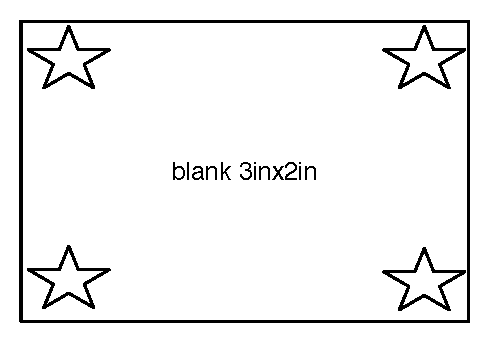
\includegraphics{figs/blank-3-2.eps}}
 \hspace{.01in}
 \subfloat[\ix]{
  \label{fig:pareto-eff:ix}
  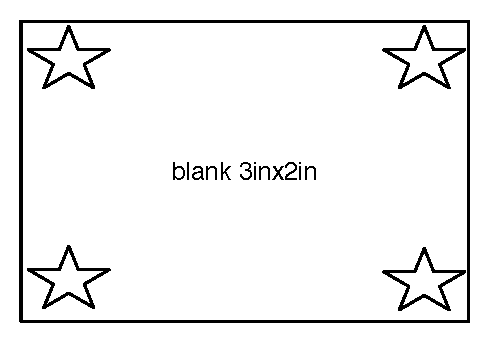
\includegraphics{figs/blank-3-2.eps}}

\caption{Pareto Efficiency measuring energy-efficiency as a function of throughput.}
\label{fig:pareto-eff}
\end{figure*}


Fig.~\ref{fig:pareto-eff} shows the Pareto-efficiency of memcache
running on both Linux  and \ix for the energy-proportionality scenario.  We report
the Energy consumed by the socket, as measured by the Intel
RAPL~\cite{missing} for static configuration that vary the number of
cores from 1 to 8 (with hyperthread enabled) and the full DVFS
frequencies of the Sandy Bridge processor, including Turbo mode.  For
simplicity, we only show the static configurations that contribute at least one point in the Pareto frontier.

Fig.~\ref{fig:pareto-eff} clearly shows that, for any given static
configuration, the energy consumed will vary noticeably as a function
of the load and that no single static configuration makes sense across
the spectrum.  Furthermore, for this workload and architecture, the
Pareto efficiency results from adding CPU at minimal frequency at
low-load, and only increasing the frequency of the CPU afterwards.
Fig.~\ref{fig:pareto-eff:linux} and Fig.~\ref{fig:pareto-eff:ix} show
that the two operating systems have different horizontal scalability
limits: memcache scales efficiently up to 8 cores on Linux where it
remains kernel-bound, but only up to 6 cores on \ix because of
application-level bottelenecks.  Next, we observe that Linux provides
a better Pareto-efficiency theoretical potential when the load is less
than XXX RPS, with \ix ouperforming Linux for all higher loads.
Clearly, the polling nature of the \ix dataplane, which is similar to
all kernel-bypass designs, only makes sense if the workload generally
has a reasonable load.  The breakeven point corresponding to XXX\% of
the peak throughput possible in the maximal configuration.  Finally,
we observe that Turbo-mode leads to a disprportional increase in
energy draw, and should be best viewed as a nice-to-have feature for
exceptional bursts in planning.


Fig.~\ref{fig:pareto-consolidation} shows the similar Pareto
efficiency in the server consolidation scenario, which combines a
CPU-intensive background job with the same latency-sensitive memcache
workload.

